\chapter{Corriente alterna}

Cuando en una gráfica de \textbf{tensión en función del tiempo} se observa un nivel de tensión por arriba del eje de abscisas, se considera positivo. Cuando está por debajo del eje, se considera negativo, y por lo tanto, representa a una corriente que está circulando en sentido contrario.
 
De esa manera, una tensión que se encuentre sin cruzar el eje en un determinado período de tiempo, se denomina \textbf{continua}. Si el sentido de la corriente cambia de forma periódica (es decir, pasa de negativa a positiva o viceversa, y se repite su forma de onda al transcurrir un determinado tiempo), se denomina \textbf{alterna}.
\begin{ejemplo}
	En las imágenes se pueden apreciar distintas variaciones de la tensión a lo largo del tiempo.
	\begin{itemize}
		\item En la \textbf{figura \ref{fig:acdc_a}}, la tensión es continua.
		\item En la \textbf{figura \ref{fig:acdc_b}}, la tensión es alterna, y tiene una forma de onda cuadrada.
		\item En la \textbf{figura \ref{fig:acdc_c}}, la tensión es alterna, y tiene una forma de onda senoidal.
		\item En la \textbf{figura \ref{fig:acdc_d}}, la tensión, si bien tiene forma de onda senoidal, es continua, porque se encuentra siempre por arriba del eje de abscisas. En otras palabras: nunca cambia su sentido, sino que sólo varía su valor de tensión.
	\end{itemize}
\end{ejemplo}

\begin{figure}[htbp]
  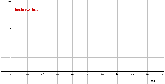
\includegraphics[scale=0.75]{images/acdc_a}
  \caption{Corriente continua}
  \label{fig:acdc_a}
\end{figure}
\begin{figure}[htbp]
  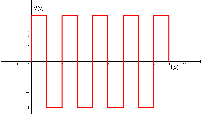
\includegraphics[scale=0.6]{images/acdc_b}
  \caption{Corriente alterna cuadrada}
  \label{fig:acdc_b}
\end{figure}
\begin{figure}[htbp]
  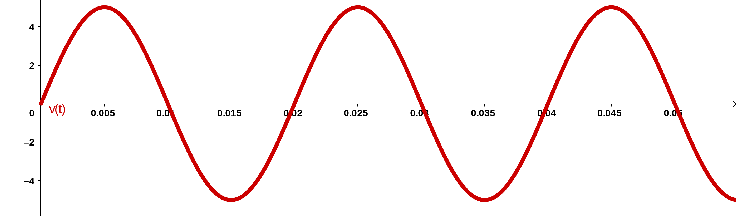
\includegraphics[scale=0.14]{images/acdc_c}
  \caption{Corriente alterna senoidal}
  \label{fig:acdc_c}
\end{figure}
\begin{figure}[htbp]
  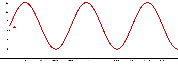
\includegraphics[scale=0.6]{images/acdc_d}
  \caption{Corriente con forma senoidal no alterna}
  \label{fig:acdc_d}
\end{figure}
Si bien existen varias formas de ondas de corriente alterna (triangular, cuadrada), la más difundida es la \textbf{forma senoidal}, que se puede apreciar en la figura \ref{fig:acdc} (C). Esto es así, porque es el voltaje que se genera en las plantas eléctricas y porque, además, permite realizar ciertos cálculos matemáticos que la explican y predicen, aunque son algo más complejos que los de corriente directa o continua.

\section{Corriente alterna senoidal}

En la figura \ref{fig:ac} se puede distinguir una onda alterna senoidal. Pueden distinguirse los siguientes parámetros:

\begin{itemize}
	\item Valor instantáneo: magnitud de una forma de onda en cualquier instante. Se han indicado como ejemplos $e_1$, $e_2$ y $e_3$.
	\item Valor pico: valor instantáneo máximo medido con respecto al nivel de 0 Volts. En la gráfica, se indicó como $Vp$. También se indicó el valor de pico negativo como $-Vp$.
	\item Valor pico a pico: tensión entre $Vp$ y $-Vp$. Es la suma entre las magnitudes de los valores de pico positivo y negativo.
	\item Ciclo: parte más pequeña de una onda hasta que comienza a repetirse.	
	\item Periodo $T$: Tiempo que dura un ciclo. En el ejemplo se tiene 3 periodos (de $O$ a $T_1$, de $T_1$ a $T_2$ y de $T_2$ a $T_3$, aunque pueden indicarse otros periodos).
	\item Frecuencia $f$: es la cantidad de ciclos que ocurren en 1 segundo. La frecuencia se mide en hertz (Hz), donde $1 Hertz = 1 ciclo por segundo$.
\end{itemize}

Del desarrollo anterior, se desprende que:
\begin{equation}
	\label{eq:frec_ciclos}
	f=\frac{1}{T}
\end{equation}
Y que:
\begin{equation}
	\label{eq:ciclos_frec}
	T=\frac{1}{f}
\end{equation}
Donde \textbf{T} se mide en segundos, y \textbf{$f$} se mide en Hz (Hertz).
\begin{figure}[htbp]
  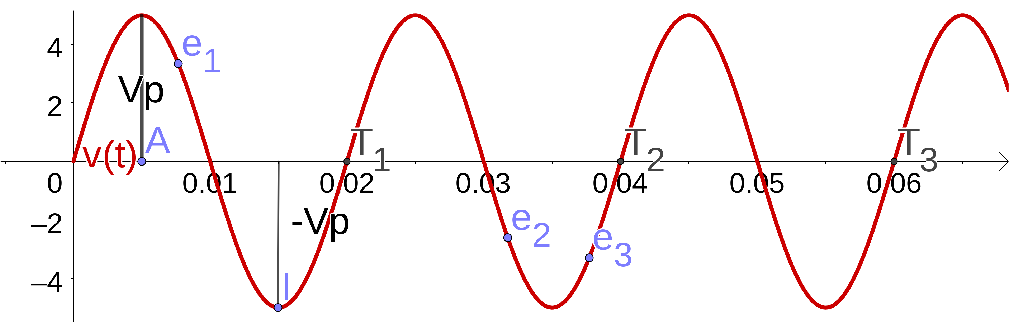
\includegraphics[scale=0.14]{images/ac}
  \caption{Corriente alterna senoidal: parámetros}
  \label{fig:ac}
\end{figure}
\begin{ejemplo}
	\label{ej:ac_argentina}
	En la figura \ref{fig:ac_argentina} se puede apreciar una onda senoidal que representa la tensión utilizada en Argentina.
	
	El valor de pico es $Vp = 311 V$ y el periodo $T = 0,02 s$.
	
	La frecuencia es $$f=\frac{1}{0,02 s}=50 Hz$$
	
	El valor de pico a pico es $$ Vpp = 2 \times 311 V = 622 V $$
\end{ejemplo}
\begin{figure}[htbp]
  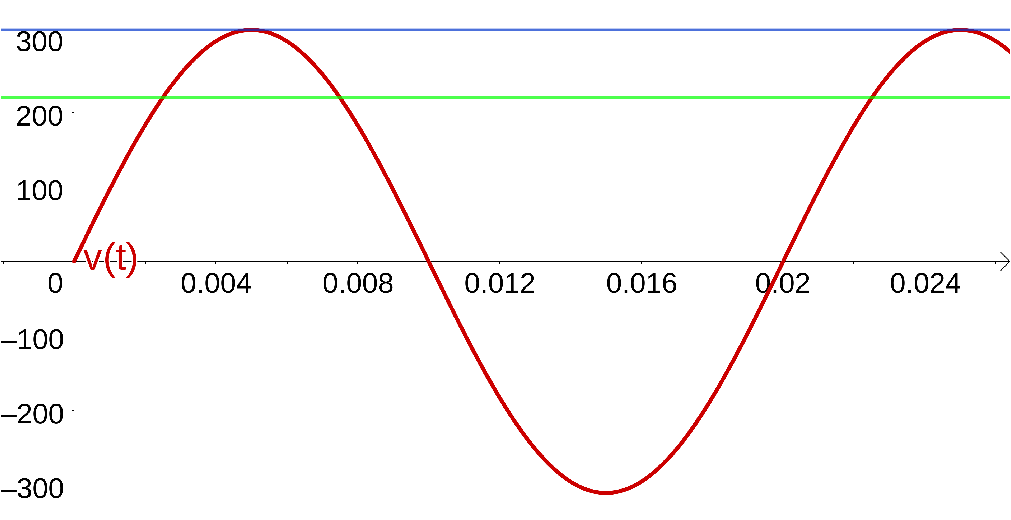
\includegraphics[scale=0.1]{images/ac_argentina}
  \caption{Corriente alterna en Argentina. En color azul, la tensión de pico y en color verde, la tensión eficaz}
  \label{fig:ac_argentina}
\end{figure}

\subsection{Definición matemática}
Si se desea considerar a la tensión (en voltios) en función del tiempo (en segundos) para una forma de onda senoidal, se deberá partir de la función $$v(\alpha) = sen (\alpha) $$
Obsérvese que en vez de utilizarse la variable $t$ (que se suele utilizar para indicar tiempo como número real), se ha definido un ángulo $\alpha$. Esto se debe a que la función senoidal está definida como el conjunto de valores que se obtienen al proyectar verticalmente un vector de radio que gira con movimiento circular uniforme alrededor de un punto fijo. La forma senoidal completa se trazará luego de haber completado una rotación de 360 grados alrededor del centro (o $2\pi$ radianes).

Suele ser más cómodo trabajar con \textbf{radianes} en vez de \textbf{grados sexagesimales} para medir los ángulos y es lo que se hará en este texto.

La idea de \textbf{proyectar verticalmente} el vector proviene de la trigonometría, ya que el $sen \alpha = \frac{\text{cateto opuesto}}{\text{radio}}$, como puede apreciarse en la figura \ref{fig:seno_triangulo}. Como el radio del vector es 1, entonces $ sen \alpha = \text{cateto opuesto} $, que es la \textbf{proyección vertical} del vector.

\begin{figure}[htbp]
  \includegraphics[scale=0.1]{images/seno_triangulo}
  \caption{Seno en un triángulo rectángulo}
  \label{fig:seno_triangulo}
\end{figure}

Un desarrollo de esta idea puede apreciarse en la figura \ref{fig:seno_proyectado}.
\begin{figure}[htbp]
%  \includegraphics[scale=1]{}
  \caption{Forma de onda senoidal a partir de la proyección de un radio versor}
  \label{fig:seno_proyectado}
\end{figure}

El vector gira con una velocidad angular $\omega$ alrededor del centro, determinada por la ecuación $$\omega = \frac{\text{distancia}}{\text{tiempo}}= \frac{\alpha}{t}$$ lo cual implica que $$ \omega t = \alpha $$

Como una vuelta completa se realiza en un periodo $T$ (que a su vez tarda 360 grados o $2 \pi$ en realizarse), se puede decir que 
$$\omega = \frac{2\pi}{T}$$ o bien, si se utiliza la ecuación \ref{eq:frec_ciclos}, $$\omega = 2\pi f$$

Volviendo a la ecuación de la tensión en función del tiempo, podría redefinirse como $$v(t) = sen (\omega t)$$, permitiendo expresar, ahora sí, la tensión en función del tiempo.

Sólo falta un detalle... debe observarse que el valor de pico de esta onda es el mismo que el del radio vector (1). Por lo tanto, la forma final de la onda seno que representa a la tensión en función del tiempo, deberá estar multiplicada por el valor de pico, de la siguiente forma: 
\begin{equation}
	\label{eq:senoidal}
	v(t) = Vp \times sen(\omega t)
\end{equation}

\subsection{Relaciones de fase}
Si la onda se desplaza $\theta$ grados, la expresión de la tensión se vuelve 
$$v=Vp \times sen (\omega t \pm \theta ) $$

Si se comparan dos ondas senoidales de la \textbf{misma frecuencia}, pueden indicarse relaciones de \textbf{adelanto} o de \textbf{atraso} de una con respecto a la otra.

\begin{ejemplo}
	En la figura \ref{fig:ejemplos_senos} puede apreciarse la función $v(t)=sen(\omega t)$ en color rojo y en color azul la función $v(t)=cos(\omega t)$. Nótese que la forma de onda es exactamente igual al seno, pero con un desplazamiento en el eje horizontal: esto es lo que habitualmente se denomina \textbf{desfasaje}. De ese modo. El coseno se podría redefinir como un seno desplazado, o viceversa: $$ sen(\alpha) = cos(\alpha - 90º) $$ $$ cos(\alpha) = sen(\alpha + 90º) $$
	Puede apreciarse en la figura, la función $sen(\omega t -90º)$ en color verde. Nótese que si el ángulo de desplazamiento es positivo, como en el ejemplo anterior, la curva se desplaza hacia la izquierda, y si el ángulo es negativo, como en este caso, el desplazamiento es hacia la derecha.
\end{ejemplo}

\begin{figure}[htbp]
  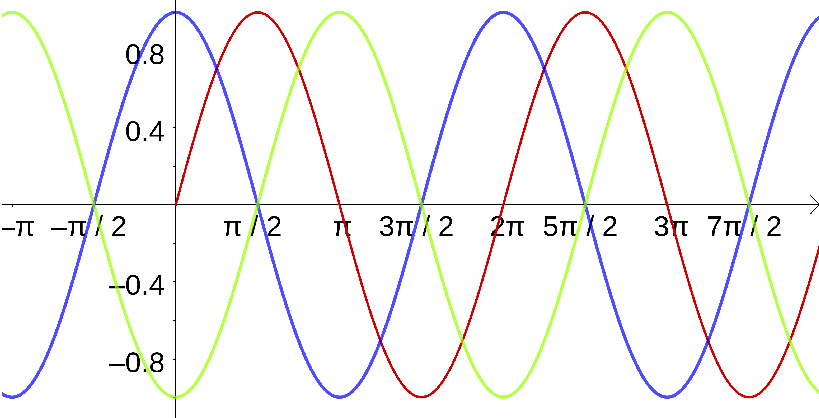
\includegraphics[scale=0.14]{images/ejemplos_senos}
  \caption{Ondas desfasadas}
  \label{fig:ejemplos_senos}
\end{figure}

\section{Valores rms}
El \textbf{valor RMS} o \textbf{valor eficaz}, es el valor de tensión o corriente alterna que produce la misma potencia que su equivalente en corriente continua.

No debe confundirse el valor eficaz con el \textbf{valor promedio}. El valor promedio de una tensión es la suma algebraica de las áreas respecto de la longitud de la curva. Si se analiza la corriente alterna senoidal, se observará que el valor promedio de tensión es de $0 V$. No ocurre lo mismo con la \textbf{tensión eficaz}.

\begin{figure}[htbp]
  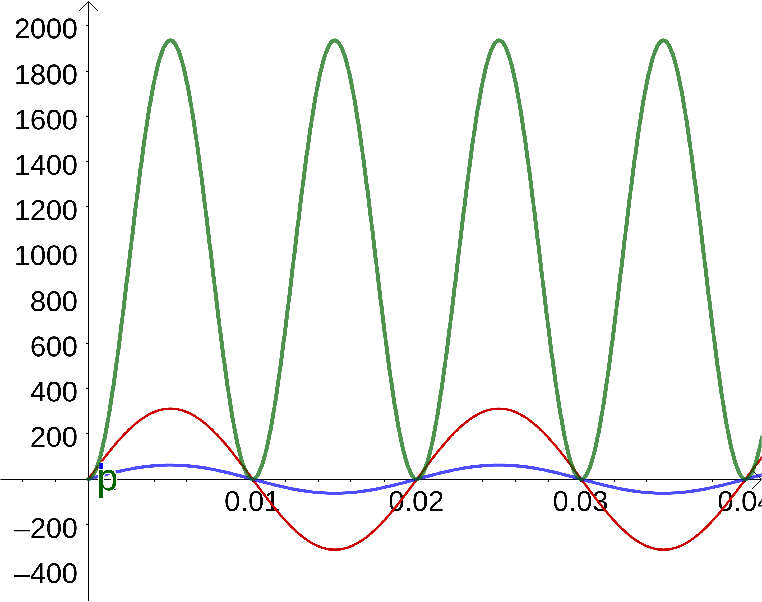
\includegraphics[scale=0.14]{images/potencia_alterna}
  \caption{Entrega de potencia en una corriente alterna senoidal}
  \label{fig:potencia_alterna}
\end{figure}

Al analizar la figura \ref{fig:potencia_alterna}, se puede observar tres ondas senoidales en fase. La más pequeña (azul), corresponde a la corriente eléctrica, medida en Amperes. La onda intermedia es la tensión (roja), expresada en Voltios. Estas ondas, poseen un semiciclo positivo y un semiciclo negativo, lo que indica un cambio en el sentido de la corriente.

La onda que toma mayor amplitud (verde), es la \textbf{potencia entregada}, calculada como el producto entre la tensión y la corriente eléctrica. Como se puede observar, todo el tiempo es positiva (excepto en los instantes 0, 0,1s y 0,2s).

Entonces, el problema de hallar la tensión eficaz, reside en observar para qué valor de tensión continua, la potencia entregada sería la misma que la de la onda más grande (verde) de la figura \ref{fig:potencia_alterna}.

A continuación se supondrá que se aplica una tensión con valor de pico $Vp$ y corriente de pico $Ip$ sobre una resistencia $R$.

\begin{eqnarray*}
	p(t)= i(t)^{2} R \\
	p(t)= [Ip sen(\omega t)]^{2} R \\
	p(t)= Ip^{2}sen^{2}(\omega t)R \\
\end{eqnarray*}
En este punto se utiliza la identidad trigonométrica $sen^{2}(\omega t) = \frac{1}{2}(1-cos(2\omega t))$.
\begin{eqnarray*}
	p(t)= Ip^{2}[\frac{1}{2}(1-cos(2 \omega t))]R \\
	p(t)=\frac{Ip^{2}R}{2}-\frac{Ip^{2}R}{2}cos(2 \omega t)
\end{eqnarray*}
Se anula el segundo término  por poseer valor medio igual a 0
 $$	p(t)=\frac{Ip^{2}R}{2} $$

Como se desea evaluar el valor de corriente continua equivalente, se supondrá que ahora se aplicó una corriente directa $I_{DC}$ a la misma carga resistiva. Su potencia $P_{DC}$ se calcularía de la siguiente forma:

$$ P_{DC} = I_{DC}^{2}R $$

Al igualar $P_{DC}$ con $p(t)$, se obtiene:
\begin{eqnarray*}
	p(t)=P_{DC} \\
	\frac{Ip^{2}R}{2}=I_{DC}^{2}R \\
	I_{DC}=\frac{Ip}{\sqrt{2}}=0,707Ip
\end{eqnarray*}

Es decir, que el valor de corriente continua equivalente de una corriente senoidal alterna es 0,707 su valor de pico. Este mismo análisis puede realizarse con la tensión, obteniendo el mismo valor.

Mediante el cálculo se puede demostrar a través de la integración, pero excede los temas de este curso.

\begin{conclusiones}
	Las siguientes ecuaciones permiten hallar valores eficaces a partir de valores de pico.
	\begin{equation}
		I_{RMS} = \frac{1}{\sqrt{2}}I_{PICO}=I_{PICO}\times 0,707
	\end{equation}
	\begin{equation}
		V_{RMS} = \frac{1}{\sqrt{2}}V_{PICO}=V_{PICO}\times 0,707
	\end{equation}
	Las siguientes ecuaciones, despejadas de las anteriores, permiten encontrar valores de pico a partir de valores eficaces.
	\begin{equation}
		I_{PICO} = \sqrt{2}I_{RMS}=I_{RMS}\times 1,414
	\end{equation}
	\begin{equation}
		V_{PICO} = \sqrt{2}V_{RMS}=V_{RMS}\times 1,414
	\end{equation}
\end{conclusiones}
\section{Fasores}
Los fasores permiten relacionar tensiones y corrientes alternas senoidales de una forma más sencilla que si se trabajara directamente con las ondas.

Como ya se sabe, una onda senoidal se define completamente por su \textbf{amplitud}, \textbf{frecuencia} y \textbf{fase}. Como se trabajará siempre con la misma frecuencia, sólo se necesitará la amplitud y la fase para poder definirlas, y ésto se puede hacer a través de vectores, que se llamarán fasores.

Un \textbf{fasor} es un número complejo que tiene como variable a su argumento.
$$ U = | U | e^{j\omega t} $$
Aplicando la fórmula de Euler en la expresión anterior, resulta,
$$ U = | U | cos (\omega t) + j|U| sen(\omega t) $$

Un fasor es un vector giratorio que permite representar una onda de corriente o tensión. El modulo del vector representa el valor eficaz de la onda, mientras que la frecuencia será la velocidad a la que giran (cuestión que será omitida, porque se supone que todos giran a la misma velocidad angular). La fase está representada por el ángulo entre fasores.

La impedancia, también es un número complejo, definido como $Z= R+j(X_L - X_C)$, y $X_L = \omega L $, $X_C = \frac{1}{\omega C}$.
\section{Potencia}
